A turtle starts at point $(0, 0)$ on the $X$-$Y$ plane. You are given a sequence of $n$ positive integers $d_1, d_2, \ldots, d_n$.

The turtle moves $d_1$ meters north, then $d_2$ meters west, $d_3$ meters south, $d_4$ meters east, and so on. After every move, its direction rotates by $90^\circ$ counter-clockwise.

\begin{center}
  \def \htmlPixelsInCm {45}
  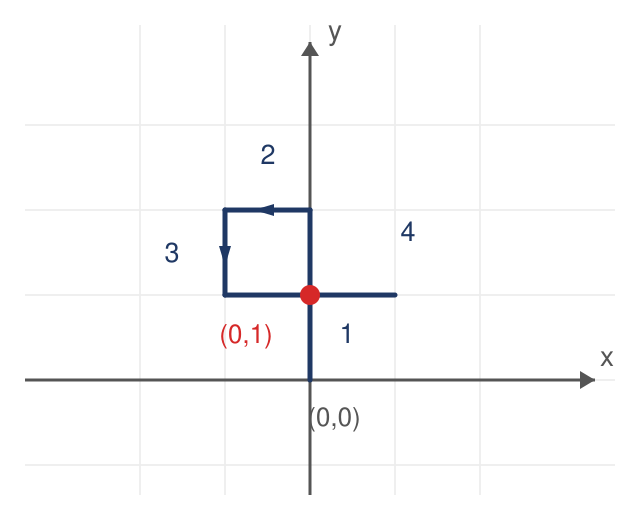
\includegraphics[width=8cm]{turtle-figure.svg} \\[4pt]
  \small{The walk of the first test case, $d = (2, 1, 1, 2)$: the fourth segment crosses the first one at $(0, 1)$.}
\end{center}

Determine whether the path drawn by the turtle intersects itself. Two path segments are considered intersecting even if they only touch at one point or overlap along a non-empty segment. The common endpoint of two consecutive moves is not considered a self-intersection.
